% ============================================================
% ============================================================
% ONERA M6 -- AERODYNAMIC GRID CONVERGENCE
% ============================================================
% ============================================================

\section[Aero.]{\textbf{Aerodynamic Grid Convergence}}


% ============================================================
% ONERA M6 -- Aerodynamic Grid Convergence: CL
% ============================================================

\begin{frame}{\small ONERA M6 -- Lift Coefficient Grid Convergence}
\scriptsize

{\centering
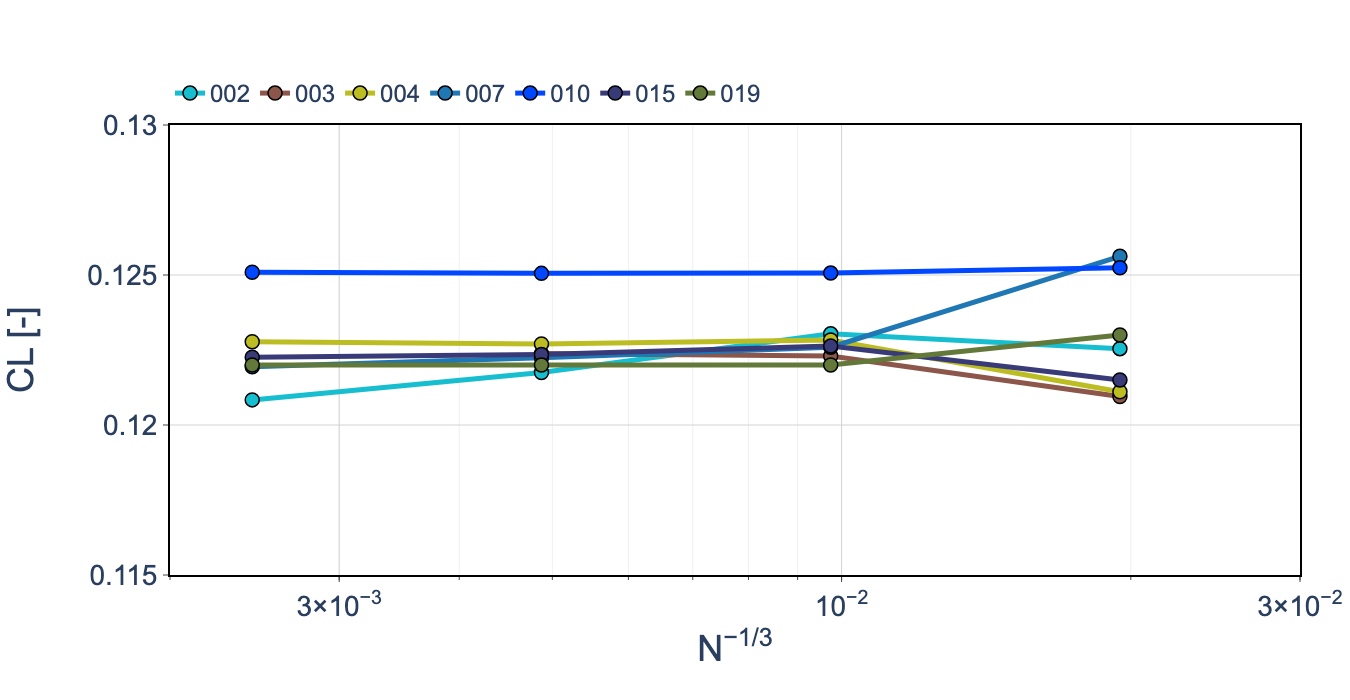
\includegraphics[width=0.48\textwidth]{FIGURES/AERODYNAMIC/tc_oneram6_cl_vs_n_1mm.png}
\hfill
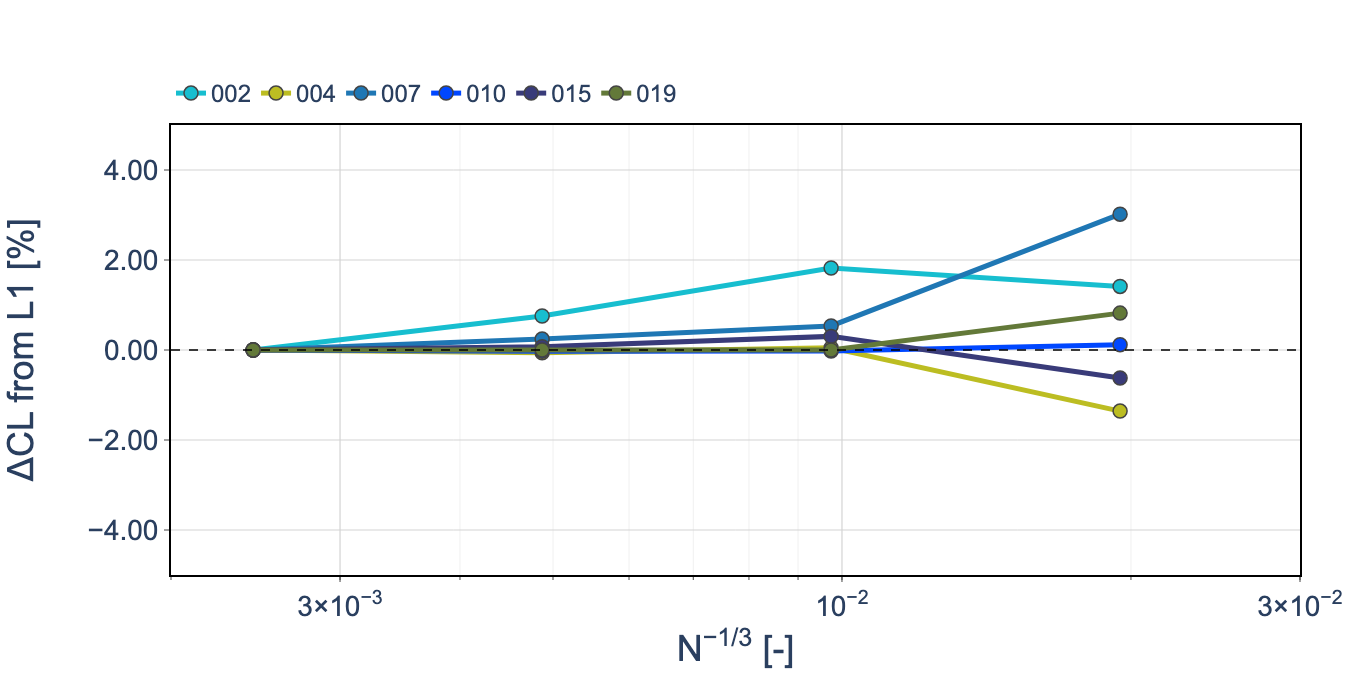
\includegraphics[width=0.48\textwidth]{FIGURES/AERODYNAMIC/tc_oneram6_cl_vs_n_1mm_relative_to_l1.png}
\par}

\vspace{0.15cm}

\begin{block}{\scriptsize Assessment}
\begin{itemize}
    \item At L1, the median lift coefficient is $C_L=0.12213$, with an IQR of $6.89\times10^{-4}$ ($0.56\%$).
    \item Coarse-grid deviations generally remain within a few percent of the corresponding L1 predictions.
    \item The code-to-code spread in $C_L$ remains small across the grid levels.
\end{itemize}
\end{block}

\end{frame}


% ============================================================
% ONERA M6 -- Aerodynamic Grid Convergence: CD
% ============================================================

\begin{frame}{\small ONERA M6 -- Drag Coefficient Grid Convergence}
\scriptsize

{\centering
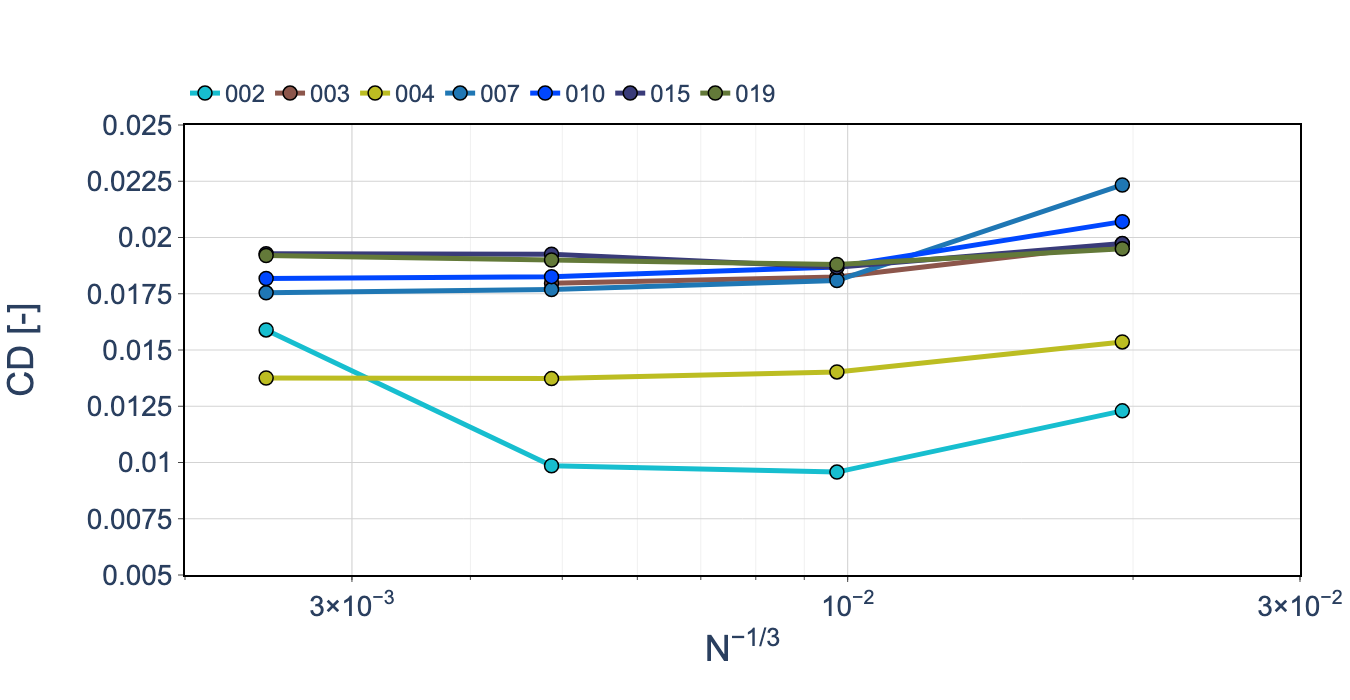
\includegraphics[width=0.48\textwidth]{FIGURES/AERODYNAMIC/tc_oneram6_cd_vs_n_1mm.png}
\hfill
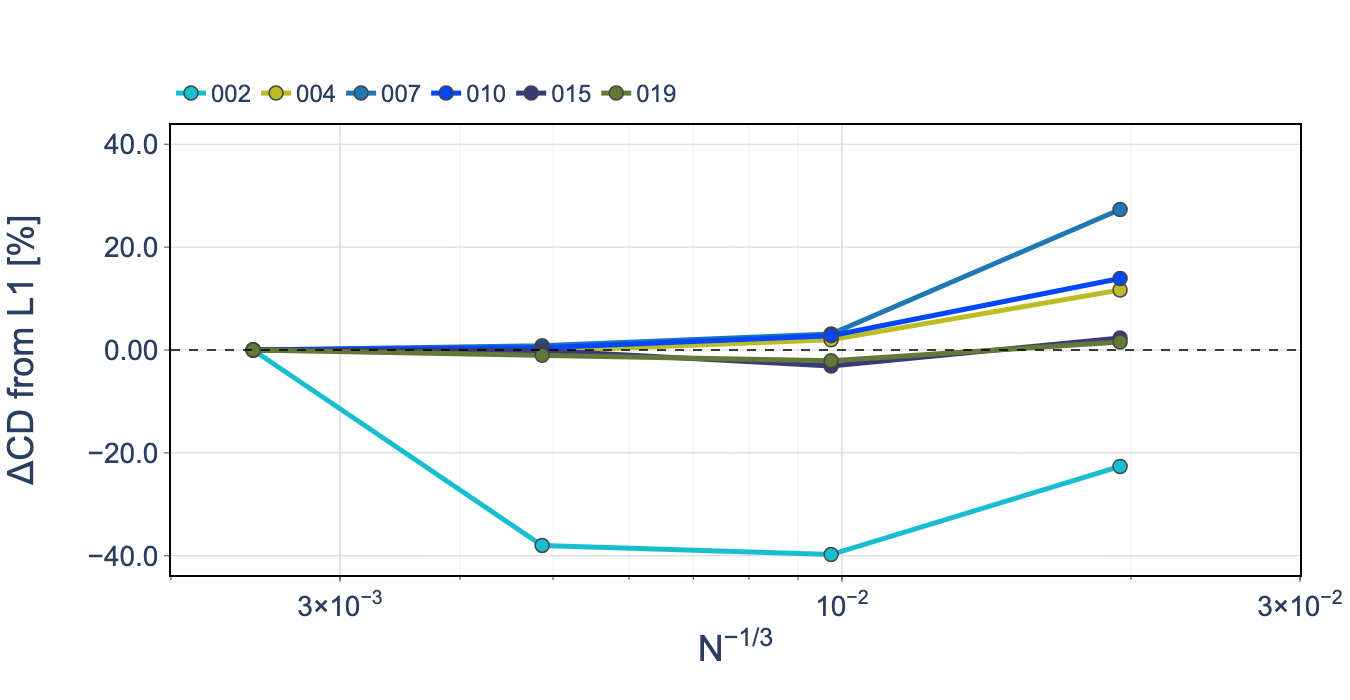
\includegraphics[width=0.48\textwidth]{FIGURES/AERODYNAMIC/tc_oneram6_cd_vs_n_1mm_relative_to_l1.png}
\par}

\vspace{0.15cm}

\begin{block}{\scriptsize Assessment}
\begin{itemize}
    \item At L1, the median drag coefficient is $C_D=0.01786$ (178.6 drag counts), with an IQR of $2.64\times10^{-3}$ (26.4 drag counts, $14.8\%$).
    \item $C_D$ exhibits considerably larger code-to-code variability than $C_L$.
    \item Several submissions show non-monotonic sensitivity to spatial grid refinement.
    \item Relative deviations from the corresponding L1 predictions reach approximately $40\%$ for selected submissions.
    \item Flow-convergence difficulties were reported for some submissions and may contribute to the observed grid sensitivity and variability in $C_D$.
\end{itemize}
\end{block}

\end{frame}


% ============================================================
% ONERA M6 -- Aerodynamic Grid Convergence: CM
% ============================================================

\begin{frame}{\small ONERA M6 -- Pitching Moment Grid Convergence}
\scriptsize

{\centering
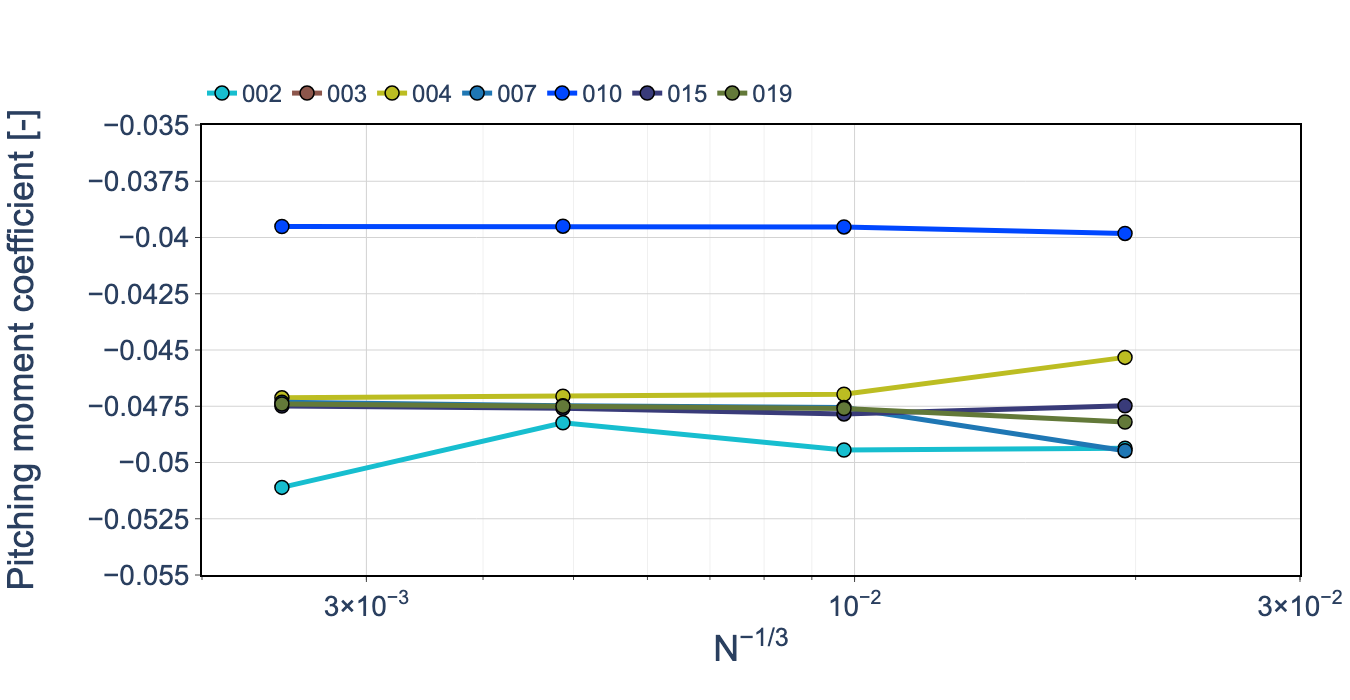
\includegraphics[width=0.48\textwidth]{FIGURES/AERODYNAMIC/tc_oneram6_cmy_vs_n_1mm.png}
\hfill
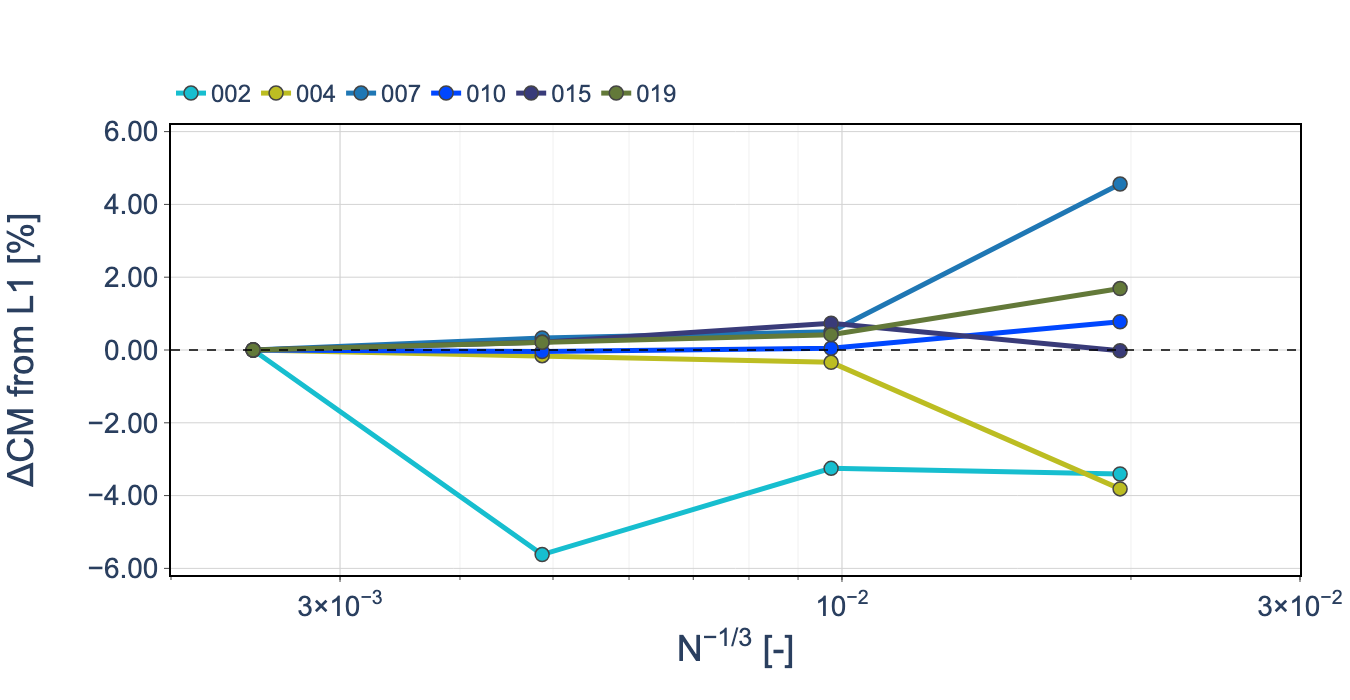
\includegraphics[width=0.48\textwidth]{FIGURES/AERODYNAMIC/tc_oneram6_cmy_vs_n_1mm_relative_to_l1.png}
\par}

\vspace{0.15cm}

\begin{block}{\scriptsize Assessment}
\begin{itemize}
    \item At L1, the median pitching-moment coefficient is $C_M=-0.04736$, with an IQR of $2.93\times10^{-4}$ ($0.62\%$).
    \item Most submissions exhibit limited sensitivity to spatial grid refinement.
\end{itemize}
\end{block}

\end{frame}


% ============================================================
% ONERA M6 -- Surface Pressure Distribution
% ============================================================

\begin{frame}{\small ONERA M6 -- Surface Pressure Distribution (L1)}
\scriptsize

% ------------------------------------------------------------
% Middle slice
% ------------------------------------------------------------
\only<1>{
\centering
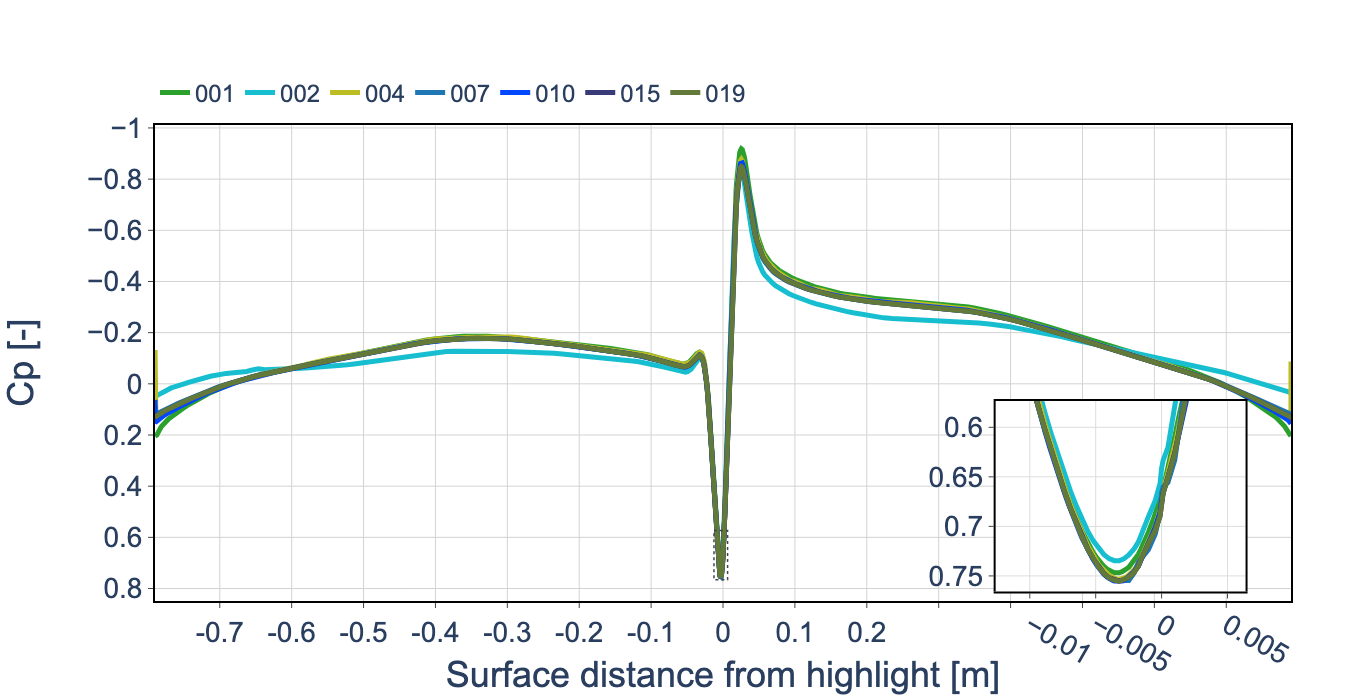
\includegraphics[width=0.62\textwidth]{FIGURES/AERODYNAMIC/tc_oneram6_L1_cp_vs_s_slice_0p75_roughness_1mm.png}

\vspace{0.05cm}

$y=0.75$ m
}

% ------------------------------------------------------------
% Inboard and outboard slices
% ------------------------------------------------------------
\only<2>{
\begin{columns}[T,onlytextwidth]

\begin{column}{0.50\textwidth}
    \centering
    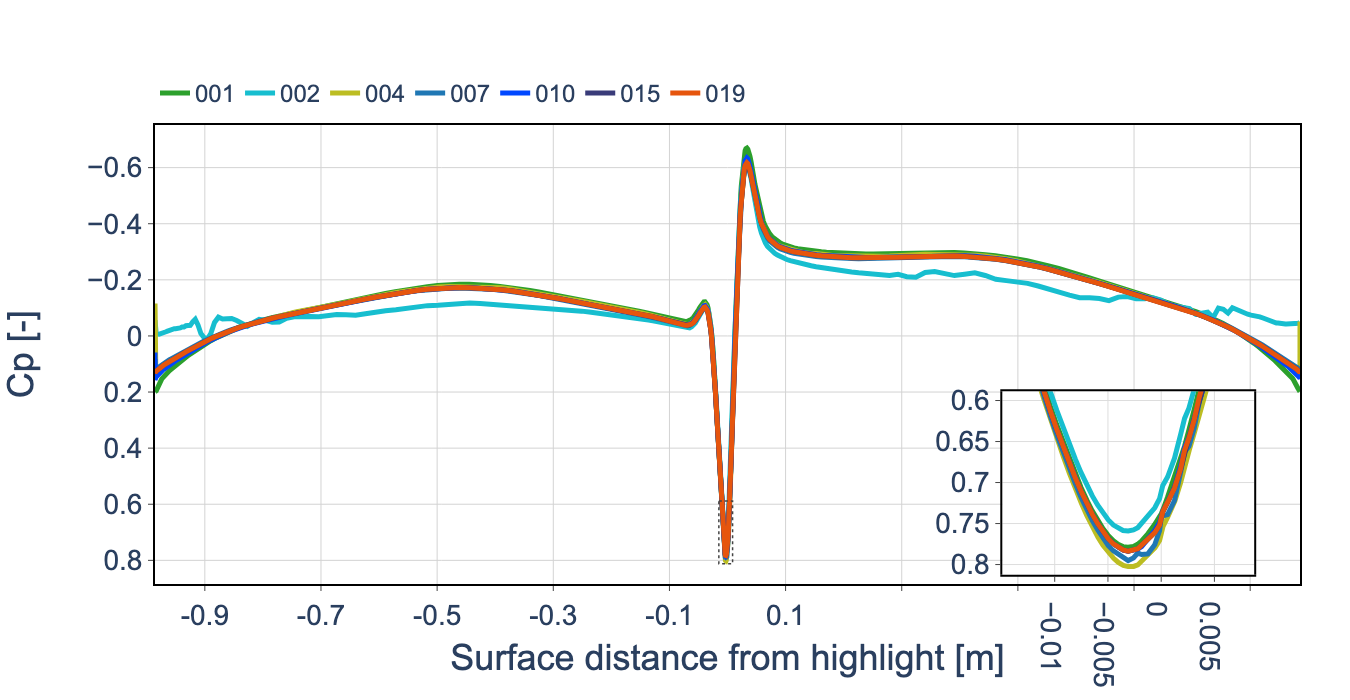
\includegraphics[width=0.94\textwidth]{FIGURES/AERODYNAMIC/tc_oneram6_L1_cp_vs_s_slice_0p1_roughness_1mm.png}

    \vspace{0.05cm}

    $y=0.10$ m
\end{column}

\begin{column}{0.50\textwidth}
    \centering
    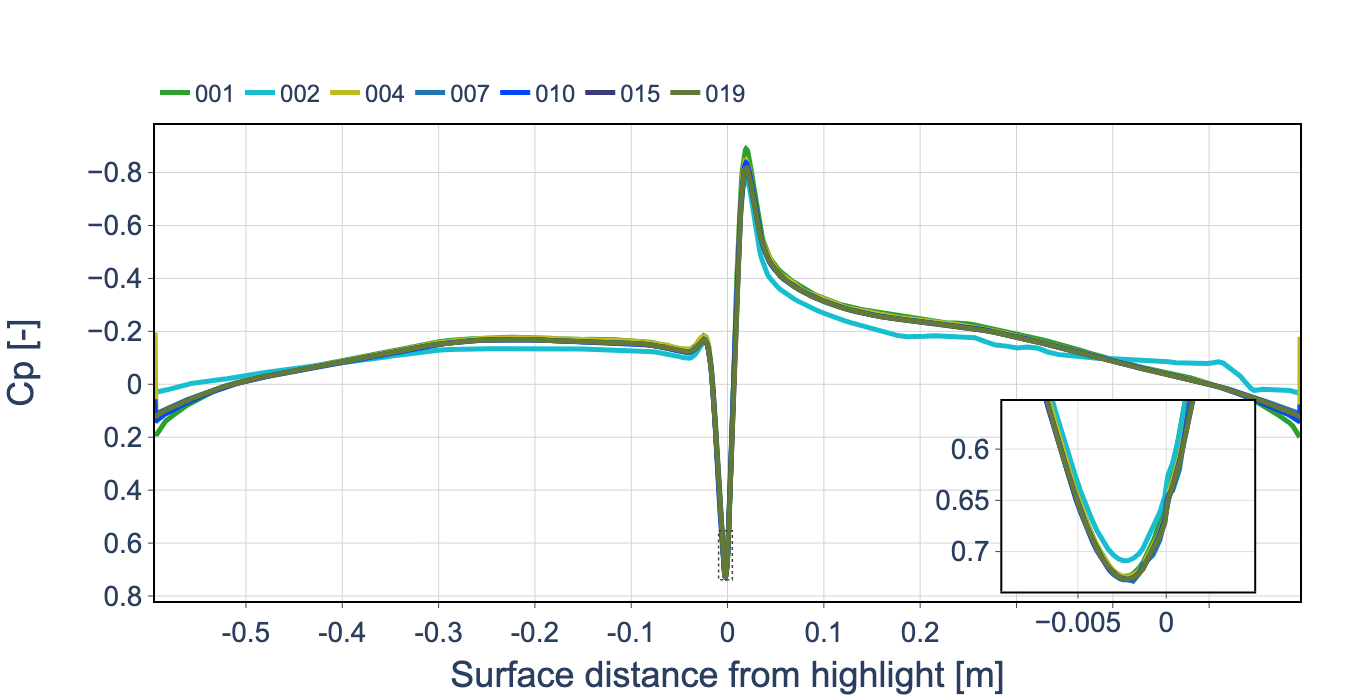
\includegraphics[width=0.94\textwidth]{FIGURES/AERODYNAMIC/tc_oneram6_L1_cp_vs_s_slice_1p4_roughness_1mm.png}

    \vspace{0.05cm}

    $y=1.40$ m
\end{column}

\end{columns}
}

\vspace{0.10cm}

\begin{block}{\scriptsize Assessment}
\begin{itemize}
    \item The submitted $C_p$ distributions are generally closely clustered across all three spanwise locations.
    \item The characteristic pressure variations associated with the leading-edge and suction-side peak are consistently captured by the participants.
    \item<2-> Overall agreement remains similar from the inboard to the outboard spanwise stations.
\end{itemize}
\end{block}

\end{frame}


% ============================================================
% ONERA M6 -- Aerodynamic Assessment Summary
% ============================================================

\begin{frame}{\small ONERA M6 -- Aerodynamic Assessment Summary}
\scriptsize

\begin{block}{\scriptsize Grid Convergence}
\begin{itemize}
    \item \textbf{$C_L$:} very weak grid sensitivity, with closely clustered predictions across the grid hierarchy.
    \item \textbf{$C_D$:} substantially greater grid sensitivity and code-to-code variability, including non-monotonic behavior for selected submissions.
    \item \textbf{$C_M$:} limited within-code grid sensitivity for most submissions.
\end{itemize}
\end{block}

\vspace{0.15cm}

\begin{block}{\scriptsize Code-to-Code Variability at L1}
\begin{center}
\begin{tabular}{lccc}
\toprule
 & \textbf{Median} & \textbf{IQR} & \textbf{Relative IQR} \\
\midrule
$C_L$ & $0.12213$  & $6.89\times10^{-4}$ & $0.56\%$ \\
$C_D$ & $0.01786$  & $2.64\times10^{-3}$ & $14.8\%$ \\
$C_M$ & $-0.04736$ & $2.93\times10^{-4}$ & $0.62\%$ \\
\bottomrule
\end{tabular}
\end{center}
\end{block}

\vspace{0.15cm}

\begin{alertblock}{\scriptsize Aerodynamic Takeaway}
The lift and pitching-moment predictions exhibit weak grid sensitivity and relatively tight code-to-code agreement for most submissions. In contrast, drag remains considerably more sensitive to both numerical implementation and spatial resolution. The $C_p$ distributions are nevertheless consistently reproduced across the three spanwise stations.
\end{alertblock}

\end{frame}


% ============================================================
% ============================================================
% END -- ONERA M6 AERODYNAMIC GRID CONVERGENCE
% ============================================================
% ============================================================